\documentclass[UTF8]{ctexart}
\usepackage{geometry}
\geometry{left=2.0cm,right=2.0cm,top=2.5cm,bottom=2.5cm}
\usepackage{amsmath}
\usepackage{cite}
\usepackage{amsthm}
\CTEXsetup[format={\large\bfseries\heiti\textbf}]{section}
\usepackage{subfigure}
\usepackage[graphicx]{realboxes}
\usepackage{caption}
\usepackage{float}

\title{不同图像识别技术的对比与探究}
\author{孟悦琦\quad 朱宸慷\quad 杨钧博\quad 李昌玟\quad 尹容乎}

\begin{document}
\maketitle

\section{背景介绍}
随着城市化进程的加速,车辆数量激增,交通管理难度加大。
为了改善城市交通状况,保障出行安全,开发自动车辆识别系统势在必行。
开发一个车辆识别系统可以提高交通管理效率、提升交通安全性。同时,车辆识别模块可以应用在诸多方面的问题上。 \par

有很多CV的方法可以进行车辆识别,这里主要可以分为传统方法和神经网络方法。
传统主要包括支持向量机、马尔可夫网络等。其特点是图像识别使用的模型相对简单、包含的参数数量有限。
同时,传统方法可能很依靠数据集的选取,在不同的数据集上可能有截然不同的表现。 \par

在CV领域,2010年出现了基于深度神经网络的模型。例如AlexNet,便是基于卷积神经网络的模型。
AlexNet具有高于传统CV方法的识别准确度\cite{AlexNet}。
之后又出现了ResNet\cite{ResNet}等方法,进一步提升其识别的准确度。
近些年,又出现了YOLO模型。
YOLO是一种划时代的单阶段目标检测算法。YOLO使用单次前馈网络即可完成检测,检测速度极快;
整图预测充分利用全局信息,检测精度高,因此被广泛使用\cite{YOLO}。
另外还有,Transformer模型,其是一种采用自注意力机制的深度学习模型,这一机制可以按输入数据各部分重要性的不同而分配不同的权重。
通过借鉴Transformer的设计思想,Google设计出ViT模型,也是一种识别准确度颇高的模型,且具有很强开创性的模型\cite{Vision_Transformers}。
在此基础上Facebook开发出LeViT模型,是其进一步分演进和发展\cite{LeViT} \par

本文将通过对比传统模型和神经网络模型,来比较分析不同模型的优劣,并分析其中的原理。

\section{数据集介绍}
现在有很多开源的数据集。考虑到本文要使用一些传统方法进行识别,我们选择的数据集不宜太大。
最终我们选择了kaggle上的Multilabel car and color dataset\footnote{可以在网站https://www.kaggle.com/datasets/julichitai/multilabel-small-car-and-color-dataset中获取}作为数据集。
在数据集中,共包含三个品牌各三种颜色的车辆图片数据。数据集的部分图片如下:

\begin{figure}[H]
    \centering
\subfigure[matiz blue]{
    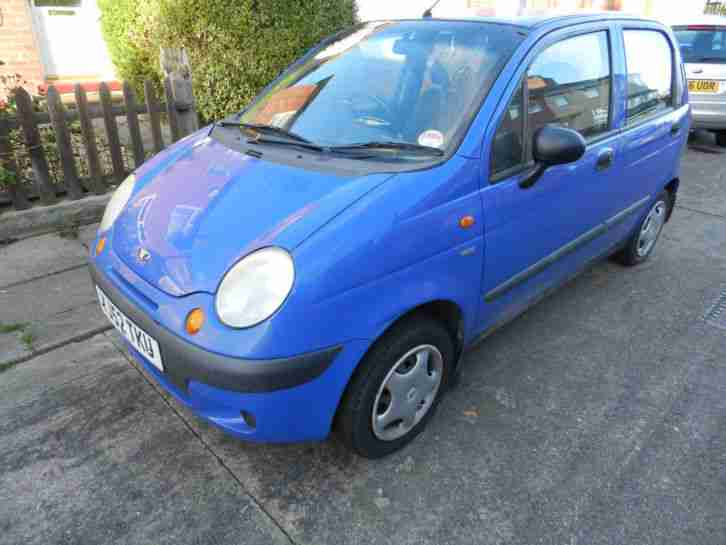
\includegraphics[width=3cm]{./dataset_graph/dataset_1.jpg}
    \label{matiz blue}
}\quad
\subfigure[tiggo black]{
    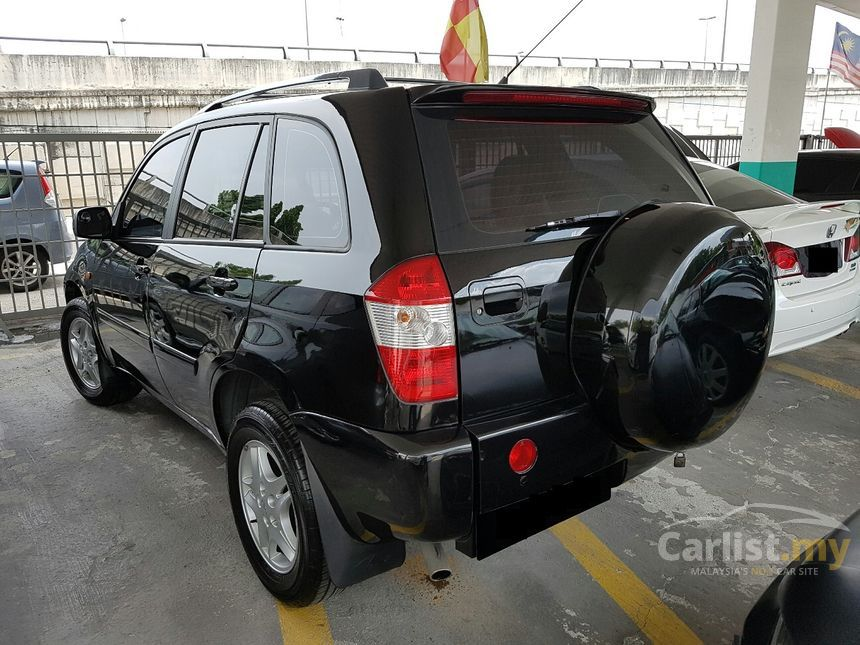
\includegraphics[width=3cm]{./dataset_graph/dataset_2.jpg}
        \label{tiggo black}
}\quad
\subfigure[rio blue]{
    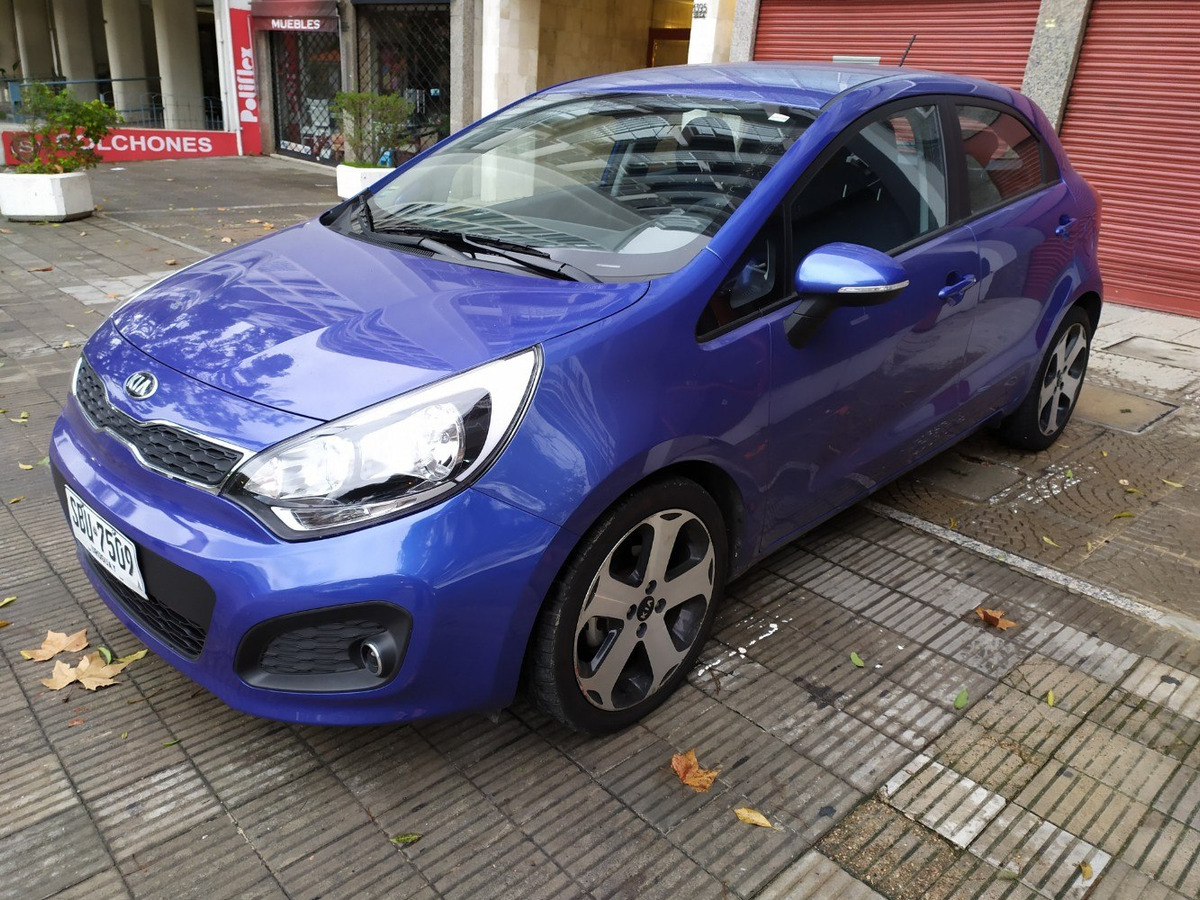
\includegraphics[width=3cm]{./dataset_graph/dataset_3.jpg}
    \label{rio blue}
}\quad
\subfigure[matiz red]{
    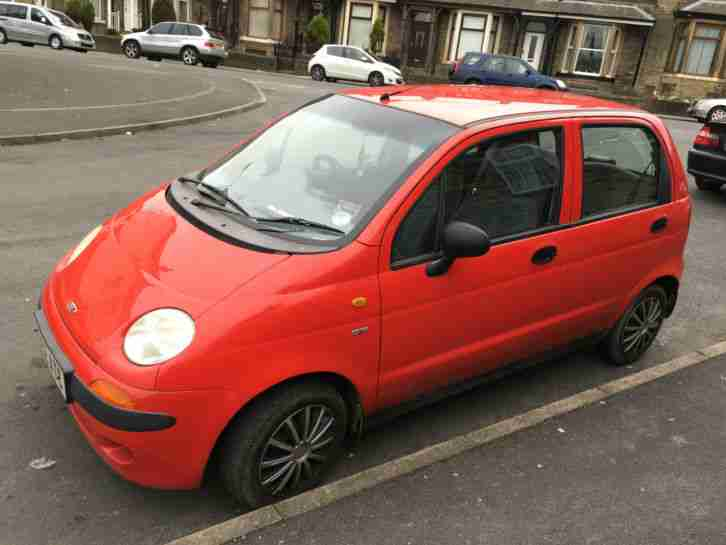
\includegraphics[width=3cm]{./dataset_graph/dataset_4.jpg}
    \label{matiz red}
}\quad
 
\caption{数据集样例}
\label{数据集样例}
\end{figure}

此数据集共有9个类,同时样本数量较少,不同品牌间视觉特征可能相近,如何提升模型泛化能力和防过拟合是关键。
此数据集很适合用来考察传统模型和神经网络之间的差别。

\section{AlexNet对数据的识别分析}
\subsection{对AlexNet的介绍}
AlexNet 是一个深度卷积神经网络,它的结构如下:\cite{AlexNet}

\begin{figure}[H]
    \centering %表示居中
    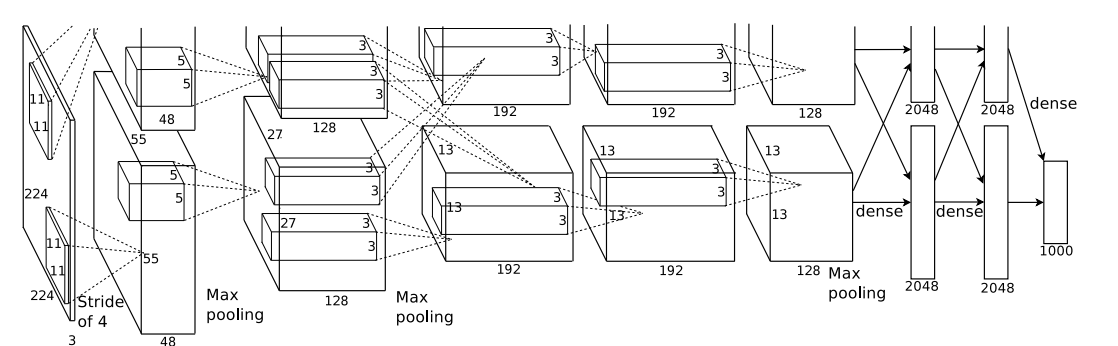
\includegraphics[height=4.5cm]{../AlexNet/AlexNet_arc.png}
    \caption{AlexNet结构}
\end{figure}

AlexNet 主要特点:\par
1. 更深的网络结构:AlexNet由 5 个卷积层、3 个全连接层和最后的 Softmax 分类层组成。 \par
2. ReLU 激活函数:AlexNet 是第一个大规模使用 ReLU 作为激活函数的网络,这加速了训练过程。 \par
3. Dropout:为了减少过拟合,AlexNet 在全连接层中使用了 Dropout。 \par
4. 局部响应归一化(LRN):在某些卷积层后使用了局部响应归一化。 \par
5. 数据增强:为了进一步减少过拟合,AlexNet 使用了图像平移、翻转和颜色变化等数据增强技术。 \par

\subsection{使用AlexNet对图像进行识别的效果分析}

训练结果如下:

\begin{figure}[H]
    \centering %表示居中
    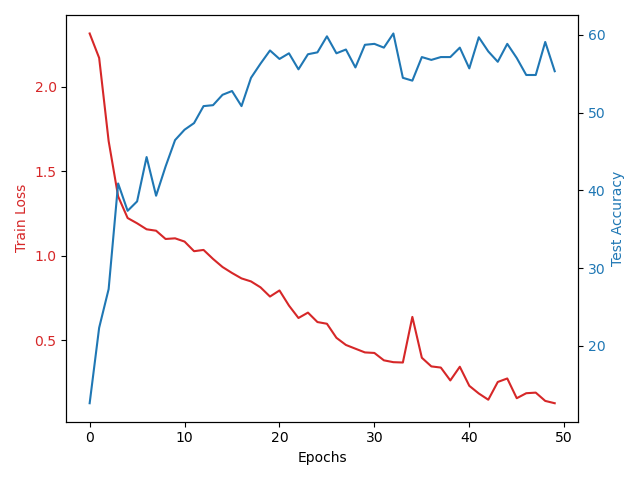
\includegraphics[height=4.5cm]{../AlexNet/AlexNet.png}
    \caption{AlexNet训练结果}
\end{figure}

在训练过程中,我们将数据集按 7:3 的比例划分为训练集和测试集。
采用 AlexNet 进行训练,训练 50 轮后,发现模型对于测试集的预测准确率不断上升,最后趋于稳定,稳定在 55\% 左右;
损失函数值也在不断下降,最终达到了 0.13。考虑到样本集中的数据量只有 2700 左右,数据量偏少,因此训练效果不是很理想。
如果增大样本集规模,模型预测的准确率应该会有进一步提升。 \par
在训练过程中发现,虽然损失函数值在下降,但是预测准确率却并未上升,有时甚至下降,这说明模型可能存在过拟合现象,这也可能是导致模型预测准确率不高的原因之一。

\newpage
\small
\bibliographystyle{IEEEtran}
\bibliography{ref}

\end{document}